\documentclass[a4j,10pt]{jarticle}
\usepackage{multicol}
\usepackage[dvipdfmx]{graphicx,xcolor}
\usepackage{caption} %multicolとfigureは上手く共存しない
%%%%% 余白の設定 %%%%%%f
\setlength{\textheight}{\paperheight}
\setlength{\topmargin}{-15.4truemm}
\addtolength{\topmargin}{-\headheight}
\addtolength{\topmargin}{-\headsep}
\addtolength{\textheight}{-20truemm}
\setlength{\textwidth}{\paperwidth}
\setlength{\oddsidemargin}{-10.4truemm}
\setlength{\evensidemargin}{\oddsidemargin}
\addtolength{\textwidth}{-30truemm}
%%%%% 行間の設定 %%%%%
\renewcommand{\baselinestretch}{.95}

\pagestyle{empty}

%%%%% 題目 %%%%%
\title{解集合プログラミングを用いたハミルトン閉路問題の解法}
%%%%% 氏名 %%%%%
\author{平手 貴大(番原研究室)}

\date{}
\begin{document}
\maketitle
\thispagestyle{empty}
\begin{multicols}{1}

%%%%%%%%%%%%%%%%%%%%%%%%%%%%%%%%%%%%%%%%%%%%%%%%%%%%%%%%%%%%%%%
\section{研究概要}
%%%%%%%%%%%%%%%%%%%%%%%%%%%%%%%%%%%%%%%%%%%%%%%%%%%%%%%%%%%%%%%
\textbf{ハミルトン閉路問題} (HCP) は,
与えられたグラフの全頂点をちょうど一度ずつ通る閉路が存在するかどうかを
判定する問題である.
ハミルトン閉路問題は代表的な NP 完全問題である.
ハミルトン路問題は,
ハミルトン閉路問題から始点と終点が一致するという閉路の条件を取り除いた
ものである.
これらの問題は,重要な工学的応用が数多く存在するため,古くから盛んに研
究されている.
例えば,数理最適化の分野で有名な巡回セールスマン問題は,グラフの辺に距
離が付随しているとき,最短距離のハミルトン閉路を求める
問題と考えることができる.
% また,ごく最近では,距離の総和が所与の閾値以下(または以上)であることを
% 制約条件として付加した
% \textbf{コスト制約付きハミルトン閉路問題}
% の解を高速に全列挙するアルゴリズムも提案されている
% 本研究では,これらの(無向グラフ上の)ハミルトン閉路問題およびその関連問
% 題を対象とする.

\textbf{解集合プログラミング}(ASP)は,論理プログラミングから派生した宣
言的プログラミングパラダイムである.
ASP言語は,一階論理に基づく知識表現言語の一種である.
%論理プログラムは ASP のルールの有限集合である.
ASP システムは論理プログラムから安定モデル意味論に基づく解集合を計算す
るシステムである.
近年,SAT技術を応用した高速 ASP システムが開発され,
スケジューリング,
プランニング,
システム生物学,
システム検証
など様々な分野への実用的応用が急速に拡大している.

\textbf{本研究の目的}は,
ASP 技術を活用し,大規模なハミルトン閉路問題および
関連問題を効率よく解くソルバーを実現することである.
ハミルトン閉路問題の ASP 符号化,
マルチショット ASPを用いた解法
を中心に研究開発を進める.
Flinders Hamiltonian Cycle Project (FHCP) で公開されている
HCP インスタンス(全1001問)を用いて実験を行い,
提案解法の有効性・実用性を評価する.

%%%%%%%%%%%%%%%%%%%%%%%%%%%%%%%%%%%%%%%%%%%%%%%%%%%%%%%%%%%%%%%
\section{研究成果}
%%%%%%%%%%%%%%%%%%%%%%%%%%%%%%%%%%%%%%%%%%%%%%%%%%%%%%%%%%%%%%%
\textbf{HCP の ASP 符号化 (卒業研究).}
ハミルトン閉路問題を解くASP符号化として,
\textsf{undirected},
\textsf{directed},
\textsf{acyclicity}
の3つを考案した.
\textsf{undirected}は,
ハミルトン閉路問題を次数制約と連結制約で簡潔に表現した符号化である.
\textsf{directed}は,
与えられた無向グラフの各辺$u-v$に対して,
2つの弧$u\rightarrow v$と$v\rightarrow u$を対応させることで有向グラフ
化して解く符号化である.
\textsf{acyclicity}は,\textsf{directed}符号化をベースに,
連結制約に代わる部分閉路禁止制約を,
ASP の組込み非閉路制約で表現した符号化である.
% 最短ハミルトン閉路問題とコスト制約付きハミルトン閉路問題については,
% 考案した3つの符号化に目的関数とコスト制約をそれぞれ追加することで自然
% に拡張できる.

% \textbf{directed 符号化の改良.}
% \textsf{directed} については,卒業研究で考案したものを改良した.
% 与えられた無向グラフの各辺に対して導入される2つの弧について,
% 高々1個がハミルトン閉路に含まれることを個数制約を使って表した.

\textbf{FHCP ベンチマーク問題集を用いた提案手法の評価.}
考案した符号化の有効性を評価するために,
Flinders Hamiltonian Cycle Project (FHCP) で公開されている
HCPインスタンス(全1001問)を用いて実験を行った.
この問題集は 2015年から2016年にかけて行われた 
FHCP Challenge と呼ばれる国際競技会で使用されたもので,
頂点数が 66個から9,528個の 充足可能な HCP インスタンスから構成されている.
実験の結果,
\textsf{directed}符号化が 875 問と最も多くの問題を解き,
他の符号化と比較してその優位性が確認できた(図~\ref{cactus}参照).
FHCP Challenge では,
整数計画ソルバー CPLEX を用いた手法が 985 問を解き優勝した.
2位〜5位の解けた問題数はそれぞれ,614 問,488 問,464 問,385 問であった.
よって,提案した\textsf{directed}符号化は,\textbf{実質2位}に相当する
性能をもつことが確認できた.

%%%%%%%%%%%%%%%%%%%%%%%%%%%%%%%%%%%%%%%%%%%%%%%
{ \centering
 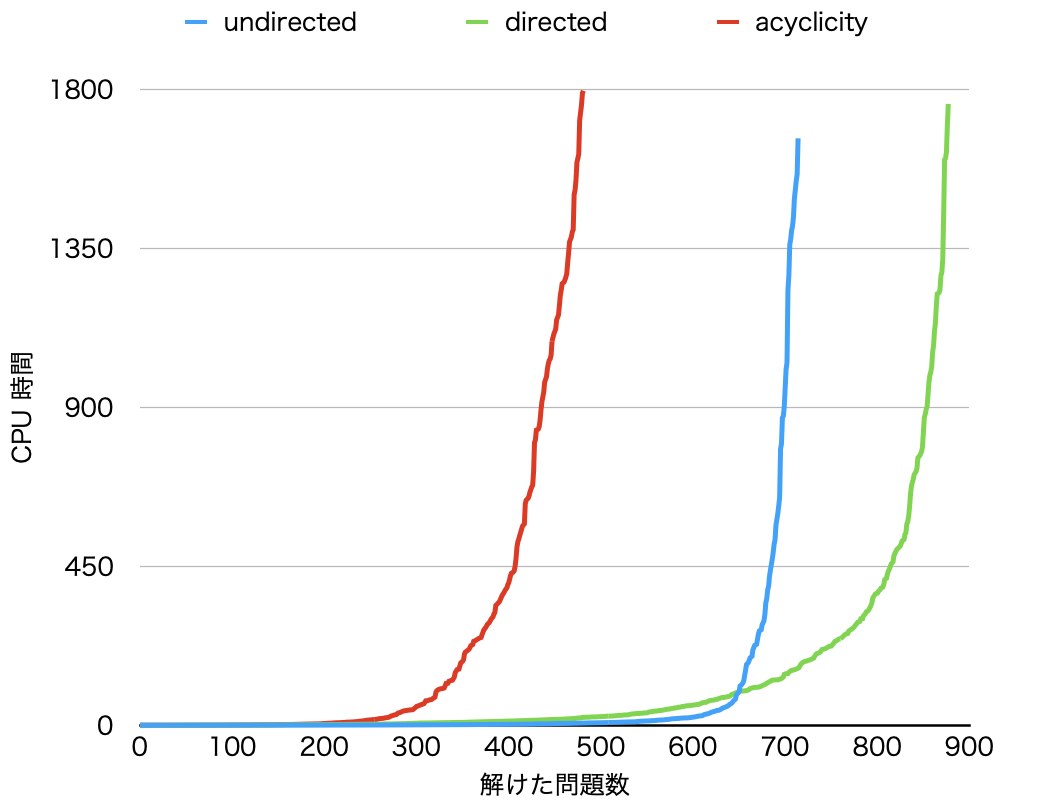
\includegraphics[width=1.0\linewidth]{cactus.png}\\
 \captionof{figure}{カクタスプロット}\label{cactus}
}
%%%%%%%%%%%%%%%%%%%%%%%%%%%%%%%%%%%%%%%%%%%%%%%

%%%%%%%%%%%%%%%%%%%%%%%%%%%%%%%%%%%%%%%%%%%%%%%%%%%%%%%%%%%%%%%
\section{まとめと今後の課題}
%%%%%%%%%%%%%%%%%%%%%%%%%%%%%%%%%%%%%%%%%%%%%%%%%%%%%%%%%%%%%%%
本稿では,解集合プログラミングを用いたハミルトン閉路問題の
解法に関して,研究概要とこれまでの研究成果を示した. 
今後の課題として,
Residue Number System やマルチショット ASP を用いた解法の考案・実装,
巡回セールスマン問題への拡張などを考えている.

%%%%%%%%%%%%%%%%%%%%%%%%%%%%%%%%%%%%%%%%%%%%%%%%%%%%%%%%%%%%%%%
\section{発表業績}
%%%%%%%%%%%%%%%%%%%%%%%%%%%%%%%%%%%%%%%%%%%%%%%%%%%%%%%%%%%%%%%
\noindent 平手貴大,宋剛秀,田村直之,番原睦則.
解集合プログラミングを用いたハミルトン閉路問題の解法に関する考察.
日本ソフトウェア科学会第38回大会講演論文集,34-L,2021年9月2日.

%%%%% 参考文献 %%%%%
% \begin{thebibliography}{10}
% \bibitem{}
% 平手貴大,宋剛秀,田村直之,番原睦則.
% 解集合プログラミングを用いたハミルトン閉路問題の解法に関する考察.
% 日本ソフトウェア科学会第38回大会講演論文集,34-L,2021年9月2日.

% \end{thebibliography}

%%%%% 本文ここまで %%%%%
\end{multicols}
\vfill
\noindent
{\gt コメント欄}
{\footnotesize
(本資料をそのまま発表者に返却します.コメント欄以外にもコメントを書いていただいてもかまいません.)}
\\
\fbox{\begin{minipage}{\textwidth}\noindent\\\\\end{minipage}}	
\end{document}
